\documentclass{article}

\usepackage{amsmath}
\usepackage{relsize}
\usepackage{tikz}

\begin{document}

\begin{center}
    \textbf{BILANGAN KOMPLEKS}
\end{center}
\leavevmode\\

Bilangan Kompleks adalah bilangan yang dapat direpresentasikan sebagai \( x + iy \), dimana $x$ dan $y$ adalah bilangan real ($R$) dan $i$ adalah suatu bilangan imaginer dimana \( i = \sqrt{-1} \) dan \( i^2 = -1 \).\\

Bilangan Kompleks biasanya ditulis dalam bentuk:
\begin{align}
    x = x + iy
\end{align}

\>dimana,
\begin{itemize}
    \item $x$ adalah bagian $Re(z)$, dan
    \item $y$ adalah bagian $Im(z)$. \\
\end{itemize}

Contoh:
\begin{align}
    z & = 6 + \sqrt{-16}
    \nonumber                            \\
      & = 6 + \sqrt{-1} \times \sqrt{16}
    \nonumber                            \\
      & = 6 + i \times 4
    \nonumber                            \\
      & = 6 + 4i
\end{align}

maka:
\begin{itemize}
    \item $Re(z) = 6$, dan
    \item $Im(z) = 4$. \\ \\ \\ \\
\end{itemize}

\newpage
\begin{center}
    \textbf{Notasi Bilangan Kompleks}
\end{center}
\leavevmode\\

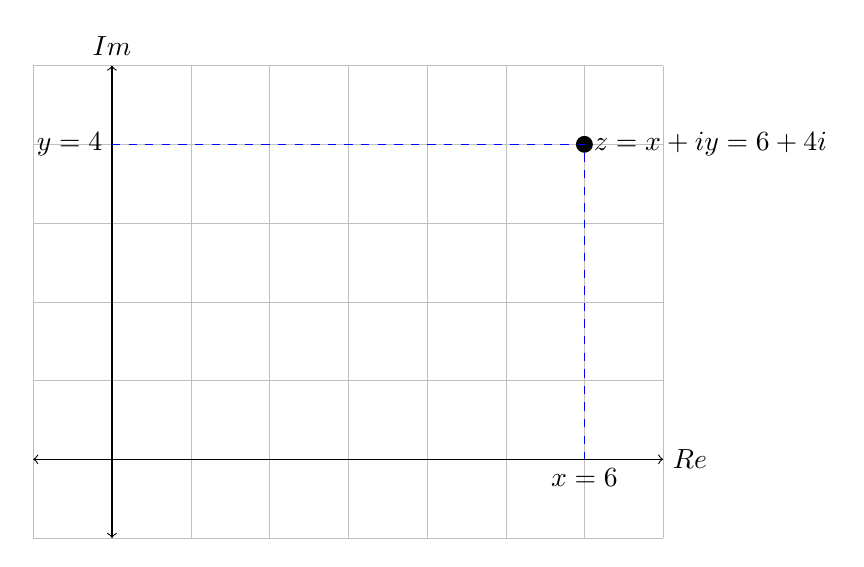
\begin{tikzpicture}
    \draw [ultra thin, lightgray] (-1,-1) grid (7,5);
    \draw [<->] (-1, 0) -- (7, 0) node[right] {$Re$};
    \draw [<->] (0, -1) -- (0, 5) node[above] {$Im$};
    \draw [black, fill = black] (6,4) circle [radius = 1 mm]
    node[black, right] {$ z = x + iy = 6 + 4i $};
    \draw [blue, dashed] (0,4) node[black, left] {$ y = 4 $}
    -| (6,0) node[black, below] {$ x = 6 $};
\end{tikzpicture}
\\ \\

Misal $ z_1 = ( x_1 , y_1 )  $ dan $ z_2 = ( x_2 , y_2 ) $, maka berlaku:

\begin{align}
    z_1 + z_2     & = ( x_1 \;,\; y_1 ) + ( x_2 \;,\; y_2 )
    \nonumber                                                       \\
                  & = ( x_1 + x_2 \;,\; y_1 + y_2 )
    \\\nonumber\\
    z_1 \cdot z_2 & = ( x_1 \;,\; y_1 ) \cdot ( x_2 \;,\; y_2 )
    \nonumber                                                       \\
                  & = ( x_1 x_2 - y_1 y_2 \;,\; x_1 y_2 + x_2 y_1 )
    \\\nonumber\\
    a \cdot z_1   & = a \cdot ( x_1 \;,\; y_1 )
    \nonumber                                                       \\
                  & = ( ax_1 \;,\; ay_1 )
\end{align}
\\ \\

\newpage
\begin{center}
    \textbf{Operasi Aritmatika Pada Bilangan Kompleks}
\end{center}
\leavevmode\\

\textbf{1.\>Penjumlahan Bilangan Kompleks\\}

Misalkan dua bilangan kompleks:
\begin{align}
    z_1 & = a + bi
    \nonumber      \\
    z_2 & = c + di
    \nonumber
\end{align}

\begin{itemize}
    \item $z_1 = 0$ jika dan hanya jika $a = 0$ dan $b = 0$
    \item $z_1 = z_2$ jika dan hanya jika $a = b$ dan $b = d$
\end{itemize}

\textbf{Contoh:}
\begin{align}
    2 + 5i = \dfrac{4}{2} + \dfrac{10}{2}i \nonumber
\end{align}
\begin{itemize}
    \item Jika $z_1 \neq z_2$ maka $z_1$ tidak dapat dibandingkan lebih besar atau lebih kecil dari $z_2$
\end{itemize}
\leavevmode
\\\\

\textbf{2.\>Perkalian bilangan kompleks dengan skalar\\}

Jika:
\begin{align}
    z_1 = (a + bi) \nonumber
\end{align}

Maka:
\begin{align}
    k \cdot z_1 = k \cdot (a + bi) = ka + kbi \nonumber
\end{align}

Contoh:
\begin{align}
    z_1 & = 2 + 5i
    \nonumber      \\
    k   & = 2
    \nonumber
\end{align}

Jawab:
\begin{align}
    k \cdot z_1 & = 2 \cdot (2 + 5i)
    \nonumber                        \\
                & = 4 + 10i
    \nonumber
\end{align}
\leavevmode
\newpage

\textbf{3.\>Perkalian dua bilangan kompleks\\}

Jika:
\begin{align}
    z_1 & = a + bi
    \nonumber      \\
    z_2 & = c + di
    \nonumber
\end{align}

Maka:
\begin{align}
    z_1 \cdot z_2 & = (a + bi)\cdot(c + di)
    \nonumber                                \\
                  & = (ac - bd) + (ad + bc)i
    \nonumber
\end{align}

Contoh:
\begin{align}
    z_1 & = 1 + 2i
    \nonumber      \\
    z_2 & = 3 + 5i
    \nonumber
\end{align}

Jawab:
\begin{align}
    z_1 \cdot z_2 & = (1 + 2i) \cdot (3 + 5i)
    \nonumber                                 \\
                  & = (3 - 10) + (5 + 6)i
    \nonumber                                 \\
                  & = -7 + 11i
    \nonumber
\end{align}

\textbf{4.\>Pembagian dua bilangan kompleks\\}

Jika
\begin{align}
    z_1 & = a + bi
    \nonumber      \\
    z_2 & = c + di
    \nonumber
\end{align}

Maka $\dfrac{z_1}{z_2}$ menyatakan pembagian bilangan kompleks dengan pembilang $z_1$ dan penyebut $z_2$. Penyebut dikalikan sekawannya $\dfrac{z_1}{z_2} \cdot \dfrac{?}{z_2}$. Agar nilai semula tidak berubah, maka pembilang juga harus dikalikan dengan bilangan yang sama: $\dfrac{z_1}{z_2} \cdot \dfrac{\overline{z_2}}{z_2}$. Sekarang pembilang bernilai riil dan pembagian dapat dilakukan.

Contoh:
\begin{align}
    z_1 & = 1 + 2i
    \nonumber      \\
    z_2 & = 2 + 3i
    \nonumber
\end{align}

Maka:
\begin{align}
    \dfrac{z_1}{z_2} & = \dfrac{1+2i}{2+3i}
    \nonumber                                                        \\
                     & = \dfrac{1+2i}{2+3i} \cdot \dfrac{2-3i}{2-3i}
    \nonumber                                                        \\
                     & = \dfrac{(2+6)+(-3+4)i}{2^2+3^2}
    \nonumber                                                        \\
                     & = \dfrac{8}{13} + \dfrac{1}{13}i
    \nonumber
\end{align}


\newpage
\begin{center}
    \textbf{Modulus Bilangan Kompleks}
\end{center}
\leavevmode\\

Modulus atau nilai absolut bilangan kompleks $ z = x + iy $, didefinisikan sebagai bilangan real tidak negatif yang merupakan panjang vektor posisi dari $z$ (jarak antara $z$ dengan pusat sumbu).
\\ \\

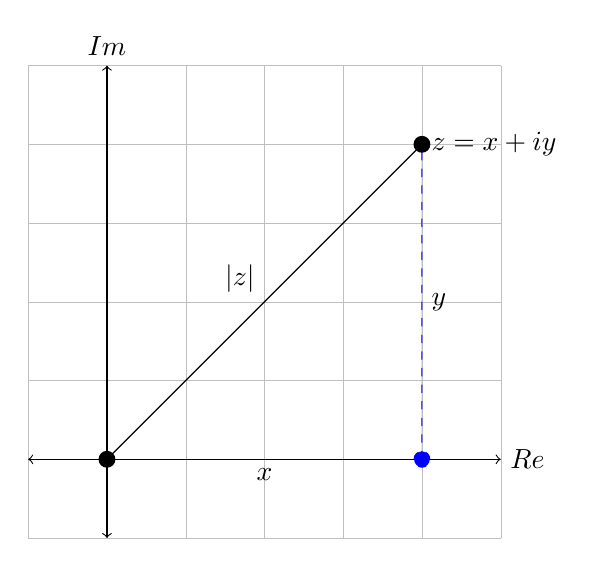
\begin{tikzpicture}
    \draw [ultra thin, lightgray] (-1,-1) grid (5,5);
    \draw [<->] (-1, 0) -- (5, 0) node[right] {$Re$};
    \draw [<->] (0, -1) -- (0, 5) node[above] {$Im$};
    \draw [black, fill = black] (4,4) circle [radius = 1 mm]
    node[black, right] {$ z = x + iy $};
    \draw [black, fill = black] (0,0) circle [radius = 1 mm] -- (4,4);
    \draw [dashed, blue, fill = blue] (4,0) circle [radius = 1 mm] -- (4,4);
    \draw (2,2) node[above, anchor=south east, black] {$|z|$};
    \draw (4,2) node[right, black] {$y$};
    \draw (2,0) node[below, black] {$x$};
\end{tikzpicture}
\\ \\

\begin{align}
    |z|         & = \sqrt{x^2+y^2}
    \\\nonumber\\
    |z_1 - z_2| & = \sqrt{(x_1-x_2)^2 + (y_1-y_2)^2}
\end{align}
\\ \\

Sifat Modulus
\begin{align}
    \bigg | \frac{z_1}{z_2} \bigg | & = \frac{|z_1|}{|z_2|}
    \\\nonumber\\
    |z_1 z_2|                       & = |z_1| \cdot |z_2|
\end{align}
\\ \\

\newpage
\begin{center}
    \textbf{Sekawan/\textit{Konjugate} Bilangan Kompleks}
\end{center}
\leavevmode\\

Misalkan $ z = x + iy $, sekawan dari $z$ (notasi = $\overline{z}$) adalah pencerminan dari $z$ terhadap sumbu real ($R$).
\\ \\

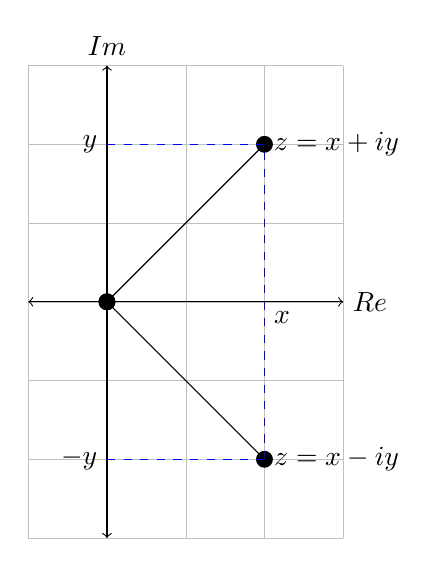
\begin{tikzpicture}
    \draw [ultra thin, lightgray] (-1,-3) grid (3,3);
    \draw [<->] (-1, 0) -- (3, 0) node[right] {$Re$};
    \draw [<->] (0, -3) -- (0, 3) node[above] {$Im$};
    \draw [black, fill = black] (2,2) circle [radius = 1 mm]
    node[black, right] {$ z = x + iy $};
    \draw [black, fill = black] (2,-2) circle [radius = 1 mm]
    node[black, right] {$ z = x - iy $};
    \draw [black, fill = black] (0,0) circle [radius = 1 mm] -- (2,2);
    \draw [black, fill = black] (0,0) circle [radius = 1 mm] -- (2,-2);
    \draw [dashed, blue] (2,-2) -- (2,2);
    \draw [dashed, blue] (0,2) node[left, black] {$y$} -- (2,2);
    \draw [dashed, blue] (0,-2) node[left, black] {$-y$} -- (2,-2);
    \draw (2,0) node[below right, black] {$x$};
\end{tikzpicture}
\\ \\ \\ \\

Sifat Sekawan/\textit{Konjugate}:
\begin{itemize}
    \item $\overline{z_1 + z_2} = \overline{z_1} + \overline{z_2}$
    \item $\overline{z_1 z_2} = \overline{z_1} \cdot \overline{z_2}$
    \item $|z| = \overline{z}$
    \item $\overline{zz} = |z|^2$
    \item $Re(z) = \dfrac{z+z}{2}$\\ \\
          $Im(z) = \dfrac{z-z}{2i}$
\end{itemize}

\newpage
\begin{center}
    \textbf{Representasi Polar}
\end{center}
\leavevmode\\

Misalkan $r$ dan adalah koordinat polar dari titik $(x, y)$ bilangan kompleks bukan nol $z = x + iy$. Karena $x = r cos \theta $ dan $y = r sin \theta$, maka bilangan Kompleks $z$ dapat
ditulis dalam bentuk polar:

\begin{align}
    z & = r(cos \theta + i sin \theta)
    \\\nonumber\\
    z & = r \angle \theta
    \\\nonumber
\end{align}

dengan,
\begin{itemize}
    \item r adalah modulus dari $z$:\\
          $ r = |z| = \sqrt{x^2+y^2} $
    \item $\theta$ adalah argumen dari $z$:\\
          $ \theta = tan^{-1} \bigg(\dfrac{y}{x}\bigg) $
\end{itemize}
\leavevmode\\

Contoh:
\begin{align}
    z = 3 + 4i \nonumber
\end{align}

Modulus:
\begin{align}
    r & = \sqrt{a^2 + b^2}
    \nonumber              \\
      & = \sqrt{3^2 + 4^2}
    \nonumber              \\
      & = 5
    \nonumber
\end{align}

Argumen:
\begin{align}
    \theta & = tan^{-1} \dfrac{b}{a}
    \nonumber                        \\
           & = tan^{-1} \dfrac{4}{3}
    \nonumber                        \\
           & = 53,1^{\circ}
    \nonumber
\end{align}

\begin{align}
    z & = 3 + 4i
    \nonumber                                      \\
      & = 5(\cos 53,1^{\circ} + \sin 53,1^{\circ})
    \nonumber                                      \\
      & = 5 \angle 53,1^{\circ}
\end{align}

\newpage
\begin{center}
    \textbf{Representasi Euler}
\end{center}
\leavevmode\\

Notasi matematis formal adalah bentuk Euler:
\begin{align}
    z = re^{i\theta} \\\nonumber
\end{align}

Identitas Euler:
\begin{align}
    e^{i\theta} = cos\theta + i sin\theta \\\nonumber
\end{align}
\leavevmode\\

Contoh:
\begin{align}
    z = 3 + 4i \nonumber
\end{align}

Modulus:
\begin{align}
    r & = \sqrt{a^2 + b^2}
    \nonumber              \\
      & = \sqrt{3^2 + 4^2}
    \nonumber              \\
      & = 5
    \nonumber
\end{align}

Argumen:
\begin{align}
    \theta & = tan^{-1} \dfrac{b}{a}
    \nonumber                        \\
           & = tan^{-1} \dfrac{4}{3}
    \nonumber                        \\
           & = 53,1^{\circ}
    \nonumber
\end{align}

\begin{align}
    z                   & = 3 + 4i
    \nonumber                                                        \\
                        & = 5e^{i 53,1^{\circ}}
    \nonumber                                                        \\
    5e^{i 53,1^{\circ}} & = 5(\cos 53,1^{\circ} + \sin 53,1^{\circ})
    \nonumber
\end{align}

\newpage
\begin{center}
    \textbf{Perkalian dan Pangkat Bentuk Exponen}
\end{center}
\begin{align}
    e^{i\theta_1} e^{i\theta_2} & = (cos\theta_1 + i sin\theta_1)(cos\theta_2 + i sin\theta_2)
    \nonumber                                                                                                                                \\
                                & =(cos\theta_1 cos\theta_2 - sin\theta_1 sin\theta_2) + i(sin\theta_1cos\theta_2 + cos\theta_1 sin\theta_2)
    \nonumber                                                                                                                                \\
                                & = cos(\theta_1 + \theta_2) + i\;sin(cos(\theta_1 + \theta_2))
    \nonumber                                                                                                                                \\
                                & = e^{i(\theta_1 + \theta_2)}
\end{align}

Maka, jika $z_1 = r_1e^{i\theta_1}$ dan $z_2 = r_2e^{i\theta_2}$, produk $z_1z_2$ memiliki bentuk eksponensial:
\begin{align}
    z_1z_2 & = r_1e^{i\theta_1} r_2e^{i\theta_2}
    \nonumber                                    \\
           & = r_1r_2e^{i\theta_1}e^{i\theta_2}
    \nonumber                                    \\
           & = (r_1r_2)e^{i(\theta_1\theta_2)}
\end{align}
\begin{align}
    \dfrac{z_1}{z_2} & = \dfrac{r_1e^{i\theta_1}}{r_2e^{i\theta_2}}
    \nonumber                                                                                                                           \\
                     & = \dfrac{r_1}{r_2} \cdot \dfrac{r_1e^{i\theta_1}}{r_2e^{i\theta_2}} \cdot \dfrac{e^{-i\theta_2}}{e^{-i\theta_2}}
    \nonumber                                                                                                                           \\
                     & = \dfrac{r_1}{r_2} \cdot \dfrac{e^{i(\theta_1-\theta_2)}}{e^{i0}}
    \nonumber                                                                                                                           \\
                     & = \dfrac{r_1}{r_2} e^{i(\theta_1-\theta_2)}
\end{align}
\begin{align}
    z^{-1} & = \dfrac{1}{z}
    \nonumber                                \\
           & = \dfrac{1e^{i0}}{re^{i\theta}}
    \nonumber                                \\
           & = \dfrac{1}{r} e^{i(0-\theta)}
    \nonumber                                \\
           & = \dfrac{1}{r} e^{-i\theta}
\end{align}
\begin{align}
    z^n & = r^n e^{in\theta}
\end{align}

\newpage
\begin{center}
    \textbf{Fungsi Kompleks}
\end{center}
\leavevmode\\

Fungsi kompleks $f(z)$ menyatakan pemetaan dari bidang kompleks asal $z$ (domain) ke bidang kompleks hasil $w$ (range) dengan suatu pola yang diatur oleh $f(z)$.
\\

Contoh (titik ke titik):
\begin{align}
    f(z)  & = 2z + 1
    \nonumber                 \\
          & = 2(x+iy) + 1
    \nonumber                 \\
          & = 2x + 2iy + 1
    \nonumber                 \\
          & = (2x + 1) + 2iy
    \\\nonumber\\
    Re(z) & = u(x,y) = 2x + 1
    \nonumber                 \\
    Im(z) & = v(x,y) = 2y
    \nonumber
\end{align}

Contoh (lintasan ke lintasan):
\begin{align}
    f(z)  & = \overline{z}
    \nonumber              \\
          & = x - iy
    \\\nonumber\\
    Re(z) & = u(x,y) = x
    \nonumber              \\
    Im(z) & = v(x,y) = -y
    \nonumber
\end{align}

Contoh (daerah ke daerah):
\begin{align}
    f(z)    & = z + 1
    \nonumber         \\
    D : |z| & <1
    \nonumber         \\
    f(z)    & = z + 1
    \nonumber         \\
    w       & = z + 1
    \nonumber         \\
    z       & = w - 1
    \nonumber         \\
    |w-1|   & < 1
    \\\nonumber
\end{align}
\\

\begin{center}
    \textbf{Titik Singular}
\end{center}
\leavevmode\\

Titik dimana $f(z)$ gagal dipetakan ke titik lain. Contoh pada fungsi \\ $f(z) = \dfrac{1}{z+1}$ gagal dipetakan pada titik asal $z=1$ karena $\dfrac{0}{0}$ tidak terdefinisi.

\newpage
\begin{center}
    \textbf{Limit Fungsi Kompleks}
\end{center}
\leavevmode\\

Konsep limit pada fungsi kompleks $f(z)$ diperluas dari limit pada fungsi real $f(x)$ sebagai:
Pada fungsi kompleks $f(z)$, $\lim_{z \to z_0} f(z)$ bernilai $L$ atau
\begin{align}
    \lim_{z \to z_0} f(z) = L
\end{align}
jika terdapat $\epsilon  > 0$ dan $\delta  > 0$ sedemikian sehingga jika ada $\epsilon$ yang memenuhi $|f(z) - L| \leq \epsilon$ , maka terilustrasi:
\begin{itemize}
    \item $|z - z_0| \leq \delta$ adalah disk dengan pusat di $z_0$ dan jari-jari $\delta$
    \item $|f(z) - L| \leq \epsilon$ adalah disk dengan pusat di $L$ dan jari-jari $\epsilon$
\end{itemize}
\leavevmode\\ \\

\begin{center}
    \textbf{Turunan Fungsi Kompleks}
\end{center}
\leavevmode\\

Perhitungan turunan $f(z)$ dapat melihat dari kemungkinan notasi $f(z)$:
\begin{itemize}
    \item $f(z)$ dinyatakan secara eksplisit peubah $z$.
    \item $f(z)$ dinyatakan : $f(z) = U(x,y) + iV(x,y)$
    \item $f(z)$ dinyatakan : $f(z) = U(i,\theta)+ iV(i,\theta)$
\end{itemize}
\leavevmode\\

$f(z)$ dinyatakan $f(z) = U(x,y) + iV(x,y)$ dapat diturunkan di $z_0 = x_0 + iy_0$ bila berlaku \textbf{Persamaan Cauchy Riemann (PCR)}:\\
\begin{align}
    Ux (x_0 + y_0) & = Vy (x_0 + y_0)
    \nonumber                                            \\
    Uy (x_0 + y_0) & = -Vx (x_0 + y_0)
    \nonumber                                            \\
    \nonumber                                            \\
    f(z_0)         & = Ux (x_0 + y_0) + i Vy (x_0 + y_0)
\end{align}
\leavevmode\\

\newpage
Contoh:

Apakah $f(z)=e^x \cdot e^{iy}$ memiliki turunan di titik $z_o = 1+i$?\\

Jawab:

$f'(1+i)$ ada jika:
\begin{align}
    Ux(1+i) & = Vy(1+i)
    \nonumber            \\
    Uy(1+i) & = -Vx(1+i)
    \nonumber
\end{align}

\begin{align}
    f(z)    & = f(z)=e^x \cdot e^{iy}
    \nonumber                             \\
            & = e^x(\cos y + i \sin y)
    \nonumber                             \\
            & = e^x \cos y + i e^x \sin y
    \nonumber                             \\
    \nonumber                             \\
    Ux(x,y) & = e^x \cos y
    \nonumber                             \\
    Uy(x,y) & = e^x (-\sin y)
    \nonumber                             \\
            & = e^x \sin y
    \nonumber                             \\
    \nonumber
\end{align}

U(x,y) dan V(x,y) memenuhi Persamaan Cauchy Riemann (PCR). Jadi $f'(1+i)$ ada:
\begin{align}
    f'(1+i) & = f'(1,1)
    \nonumber                       \\
            & = e'cos 1 + i e'sin 1
    \nonumber                       \\
    \nonumber
\end{align}


$f(z)$ dinyatakan sebagai $f(z) = U(i,\theta)+ iV(i,\theta)$

PCR dalam koordinat polar:
\begin{align}
    Ur                  & = \dfrac{1}{r}V\theta
    \nonumber                                   \\
    \dfrac{1}{r}U\theta & = -Vr
    \nonumber                                   \\
    \nonumber
\end{align}

Turunan dari f(z) dinyatakan :
\begin{align}
    f'(z) = e^{-i\theta}(Ur+iVr)
\end{align}

\newpage
\textbf{Metode Milne-Thomson}
\leavevmode\\

Jika fungsi terurai $f(x+iy)=u(x,y) + iv(x,y)$  differentiable atau holomorfik, maka $f(x+iy)$ dapat dijadikan bentuk kompak $f(z)$.

\begin{itemize}
    \item Tentukan $f'(x+iy)$ yaitu $f'(x+iy) = \dfrac{\partial u}{x} + i \dfrac{\partial v}{x}$
    \item Ditinjau suku $\dfrac{\partial u}{x}$
    \item Substitusi $\dfrac{\partial u}{x} \rightarrow  f'(z), x \rightarrow z$ dan $y \rightarrow 0$
    \item Selesaikan $f'(z)$ untuk memperoleh $f(z)$
    \item Cari konstanta $c$ pada $f(z)$ dengan substitusi $z = x +iy$ pada $f(z)$ dan membandingkannya dengan $f(x+iy)$ semula.
\end{itemize}

Contoh:
\begin{align}
    f(z) & = e^x \cos y + i e^x \sin y
    \nonumber
\end{align}
\begin{align}
    u_x & = e^x \cos y  & v_x & = e^x \sin y
    \nonumber                                \\
    u_y & = -e^x \sin y & v_y & = e^x \cos y
    \nonumber
\end{align}
\begin{align}
    u_x & = v_x
    \nonumber    \\
    u_y & = -v_y
    \nonumber
\end{align}
\begin{align}
    f(z) & = e^x \cos y + i e^x \sin y
    \nonumber                          \\
         & = e^x (\cos y + i \sin y)
    \nonumber                          \\
         & = e^x \cdot e^iy
    \nonumber                          \\
         & = e^{x+iy}
    \nonumber                          \\
         & = e^z
    \nonumber\
\end{align}

$u_x  = e^x cos y \rightarrow$ ganti $x$ dengan $z$

$y$ dengan $0$
\begin{align}
    f'(z) & = e^z cos 0
    \nonumber                            \\
          & = e^z \rightarrow f(z) = e^z
    \nonumber
\end{align}


\newpage
Aturan penurunan pada fungsi riil berlaku pada fungsi kompleks. Jika $f(z)$ dan $g(z)$ adalah dua fungsi kompleks, maka:
\begin{itemize}
    \item penjumlahan
          \begin{align}
              \frac{d}{dz}(f(z)+g(z)) & = f'(z) + g'(z)
          \end{align}
    \item perkalian skalar
          \begin{align}
              \frac{d}{dz}(kf(z)) & = kf'(z)
          \end{align}
    \item aturan rantai
          \begin{align}
              \frac{d}{dz}(f(g(z))) & = f'(g(z)) g'(z)
          \end{align}
    \item aturan perkalian
          \begin{align}
              \frac{d}{dz}[f(z)g(z)] & = f'(z)g(z) + g'(z)f(z)
          \end{align}
    \item aturan pembagian
          \begin{align}
              \frac{d}{dz}\frac{f(z)}{g(z)} & = \frac{f'(z)g(z) - g'(z)f(z)}{g^2(z)}
          \end{align}
\end{itemize}


\newpage
\begin{center}
    \textbf{Persamaan Cauchy-Riemann (PCR)}
\end{center}
\leavevmode\\

Syarat terpenuhi Persamaan Cauchy-Riemann (PCR):\\

Diketahui:
\begin{align}
    f(x,y) = x + iy
    \nonumber
\end{align}

Memenuhi Persamaan Cauchy-Riemann (PCR), jika:
\begin{align}
    \dfrac{\partial U}{\partial x} = \dfrac{\partial V}{\partial y}
\end{align}
\begin{center}
    dan
\end{center}
\begin{align}
    \dfrac{\partial U}{\partial y} = -\dfrac{\partial V}{\partial x}
\end{align}

dimana:
\begin{itemize}
    \item U adalah bagian $Re f(x,y)$, dan
    \item V adalah bagian $Im f(x,y)$.
\end{itemize}

Jika PCR tidak terpenuhi maka $f(x,y)$ tidak differentiable, atau $f'(x,y)$ tidak ada.
\leavevmode\\ \\

Contoh:

Tentukan turunan fungsi $f(x,y) = x^2 -y^2 + i2xy$
\begin{align}
    U_x & = 2x  & V_x & = 2y
    \nonumber                \\
    U_y & = -2y & V_y & = 2x
    \nonumber
\end{align}

PCR terpenuhi
\begin{align}
    f'(x+iy) & = U_x +iV_x
    \nonumber              \\
             & = 2x +i2y
    \nonumber              \\
             & = 2(x+iy)
    \nonumber
\end{align}

Jika dilakukan pada bentuk kompak:
\begin{align}
    f(x+iy)  & = x^2 -y^2 + i2xy
    \nonumber                    \\
    f(z)     & = z^2
    \nonumber                    \\
    f'(x+iy) & = 2(x+iy)
    \nonumber                    \\
    f'(z)    & = 2z
    \nonumber
\end{align}
\leavevmode\\ \\


\newpage
\begin{center}
    \textbf{Fungsi Harmonik}
\end{center}
\leavevmode\\

Misalkan $u(x,y)$ adalah fungsi 2 peubah $u(x,y)$ dikatakan fungsi harmonik jika $u_{xx} + u_{yy}$. Buktikan bahwa $u(x,y) = 3x^2 - 3y^2 + 2x$ adalah harmonik?
\begin{align}
    u_x             & = 6x-0+2   & u_y    & = -6y
    \nonumber                                     \\
    u_{xx}          & = 6        & u_{yy} & = -6
    \nonumber                                     \\
    \nonumber                                     \\
    u_{xx} + u_{yy} & = 6 + (-6)
    \nonumber                                     \\
                    & = 0
    \nonumber                                     \\
                    & (harmonik)
    \nonumber
\end{align}

Contoh:

$H(x,y) =2x^3 -kyx^2$ tentukan nilai $k$ sehingga $H(x,y)$ menjadi fungsi harmonik
\begin{align}
    H_x    & = 6x^2-ky^2 & H_y    & = 0-2kxy
    \nonumber                                \\
    H_{xx} & = 12x       & H_{yy} & = -2kx
    \nonumber
\end{align}

Agar harmonik
\begin{align}
    H_{xx} + H_{yy} & = 0
    \nonumber               \\
    12x + (-2kx)    & = 0
    \nonumber               \\
    12 - 2k         & = 0
    \nonumber               \\
    -2k             & = -12
    \nonumber               \\
    k               & = 6
    \nonumber
\end{align}

\newpage
\begin{center}
    \textbf{Fungsi Analitik}
\end{center}
\leavevmode\\

Fungsi $f(z)$ disebut analitik pada $D$ (himpunan buka) bila $f'(z)$ ada untuk $z \epsilon D$ atau $f(z)$. Berlaku PCR untuk $z \epsilon D$.
\begin{itemize}
    \item \textbf{Differentiable} $\rightarrow$ Fungsi $f(z)$ dikatakan terdifferentiable di $z=z_0$ jika $f'(z)$ ada untuk $z=z_0$.
    \item \textbf{Analitik} $\rightarrow$ Fungsi $f(z)$ dikatakan analitik pada suatu titik $z$ jika $f'(z)$ ada untuk $z=z_0$ dan sekitarnya.
\end{itemize}

Contoh:

Periksa apakah $f(z)$ fungsi analitik pada $D$.
\begin{align}
    f(z) & = \dfrac{z^2 + 1}{z - 2}
    \nonumber                       \\
    D    & = |z + 1| < 1
    \nonumber
\end{align}

\begin{align}
    f'(z) & = \dfrac{g'h - h'g}{h^2}
    \nonumber                        \\
    g     & = z^2+1
    \nonumber                        \\
    h     & = z-2
    \nonumber
\end{align}

$f(z)$ tidak ada $\rightarrow$ $f'(z)$ tidak ada.
\begin{align}
    z + 1    & < 1
    \nonumber      \\
    z - (-1) & < 1
    \nonumber      \\
    z - z0   & < r
    \nonumber
\end{align}

Himpunan $z$ yang jaraknya terhadap $z_0$ kurang dari $r$.
\\

Misal  $u(x,y)$ dan  $v(x,y)$ pada $D$ dan berlaku PCR maka $v(x,y)$ disebut konjugate (sekawan) harmonik dari $u(x,y)$ atau sebaliknya.
\begin{itemize}
    \item $u(x,y)$ dan $v(x,y)$ masing-masing punya fungsi harmonik.
    \item $u_x = v_y$ dan $u_y = -v_x$
\end{itemize}


\newpage
\begin{center}
    \textbf{Sekawan Harmonik}
\end{center}
\leavevmode\\

PCR digunakan untuk mencari Sekawan Harmonik.\\

Misal:
\begin{align}
    f(x + iy) = xy + iV(x, y)
    \nonumber
\end{align}

Tentukan $V(x,y)$ sekawan harmonik dari $U = xy$.\\
Jawab:
\begin{align}
    U_x           & = y    \; & \;   U_y    & = x
    \nonumber                                     \\
    U_{xx}        & = 0    \; & \;   U_{yy} & = 0
    \nonumber                                     \\\nonumber\\
    U_{xx}+U_{yy} & =0
    \nonumber                                     \\
    0 + 0         & =0
    \nonumber
\end{align}
Terbukti Harmonik.\\

\begin{align}
    U_x & = y                                \; & \;   U_y & = x
    \nonumber                                                                                 \\
    V_x & = \dfrac{\partial V}{\partial x}   \; & \;   V_y & = \dfrac{\partial V}{\partial y}
    \nonumber
\end{align}

PCR Syarat 1:
\begin{align}
    U_x & = Vy
    \nonumber                              \\
    y   & = \dfrac{\partial V}{\partial y}
    \nonumber                              \\
    V   & = \dfrac{1}{2} y^2 + g(x)
    \nonumber
\end{align}

Turunkan $V$ yang baru diperoleh terhadap $x$:
\begin{align}
    \dfrac{\partial V}{\partial x} = g'(x)
    \nonumber
\end{align}

PCR Syarat 2:
\begin{align}
    U_y & = -Vx
    \nonumber                               \\
    x   & = -\dfrac{\partial V}{\partial x}
    \nonumber                               \\
    x   & = g'(x)
    \nonumber
\end{align}

\begin{align}
    g'(x) & = x
    \nonumber                      \\
    g(x)  & = \dfrac{1}{2} x^2 + c
    \nonumber
\end{align}

Sehingga:
\begin{align}
    V & = \dfrac{1}{2} x^2 + \dfrac{1}{2} y^2 + c
    \nonumber
\end{align}

dengan c suatu konstanta.


\newpage
\begin{center}
    \textbf{Integral Kompleks}
\end{center}
\leavevmode\\

\textbf{Lintasan 1}
\\

Misal $z(t) : 1 \rightarrow C$ merupakan fungsi kompleks dengan domain real, $1=[a,b]$, maka fungsi $z(t)$ dinyatakan:
\begin{align}
    z(t) & = x(t) + iy(t)
    \nonumber              \\
         & a \leq t \leq b
    \nonumber
\end{align}


$z(t)$ merupakan lintasan dari $A$ ke $B$. Rotasi : $Z$\\

Contoh:

Gambarkan lintasan  $C$ untuk $-1 \leq t \leq 1$ yang dinyatakan
\begin{align}
    z(t) & = t + it^2
    \nonumber                     \\
    x(t) & = t \rightarrow y= x^2
    \nonumber                     \\
    y(t) & = t^2
    \nonumber
\end{align}
\leavevmode\\

\textbf{Lintasan 2}
\\

Turunan 2 integral dari persamaan lintasan dinyatakan sebagai berikut:
$z(t) =x(t) +i y(t) ; a \leq t \leq b$
\begin{align}
    \dfrac{dz}{dt}         & = z'(t)
    \nonumber                                                                   \\
    \dfrac{dz}{dt}         & = x'(t) + iy'(t)
    \nonumber                                                                   \\
    \int_{a}^{b} z(t) \,dt & =\int_{a}^{b} x(t) \,dt + i \int_{a}^{b} y(t) \,dt
    \nonumber
\end{align}
\leavevmode\\

Contoh:

Hitung turunan dan integral dari persamaan lintasan berikut:
\begin{align}
    z(t) & = t + it^2
    \nonumber            \\
    -1   & \leq t \leq 1
    \nonumber
\end{align}
\begin{align}
    z'(t)                   & = 1 + 2it
    \nonumber                                                               \\
    \int_{-1}^{1} t(t) \,dt & = \int_{-1}^{1} [t + it^2] \,dt
    \nonumber                                                               \\
                            & = [\dfrac{1}{2}t^2 + \dfrac{i}{3}t^3]_{-1} ^1
    \nonumber                                                               \\
                            & = \dfrac{2}{3}i
    \nonumber
\end{align}
\leavevmode\\

\textbf{Jenis Lintasan:}
\begin{enumerate}
    \item Lintasan buka : Bila ujung lintasan tidak berimpit
    \item Lintasan tutup : Bila ujung lintasan berimpit (Sederhana \& tidak sederhana)
\end{enumerate}
\leavevmode\\

\textbf{Integral Lintasan:}

Integral dari fungsi kompleks $f(z)$ atas lintasan $C$ disebut integral lintasan atau integral garis atau integral sountour dan dinyatakan:
\leavevmode\\ \\

\textbf{Integral tergantung lintasan 1:}
\begin{enumerate}
    \item Nyatakan lintasan C dalam $z(t) =t +it2 ; -1 \leq t \leq 1$
    \item Cari turunan $z(t) z'(t)$
    \item Substitusi fungsi $f(z)$ terhadap fungsi $z (t)  f[z(t)]$
    \item Integrasikan  $f[z(t)] z'(t)$ terhadap $t$
\end{enumerate}
\leavevmode\\

\textbf{Titik Interior:}

Titik to disebut titik interior dari lintasan tutup $C$ bila terdapat lingkungan dari to yang termuat di dalam $C$.

Lintasan tutup $C$ arah positif : bila berjalan menyusuri lintasan maka daerah yang dilingkupi oleh $C$ terletak disebelah kiri.
\leavevmode\\

\newpage
\textbf{Integral Cauchy}

Misal lintasan $C$ tutup dengan arah berlawanan jarum jam (arah positif),  $z_0$ : interior dari $C$ dan $f(z)$ analitik pada daerah yang dilingkupi oleh $C$ maka integral cauchy:
\leavevmode\\

Jika:
\begin{enumerate}
    \item $C$ lintasan tutup arah $(t)$
    \item $g(z) = \dfrac{f(z)}{z-z_0} , f(z)$ analitik di lintasan $C$
    \item $z_0$ titik interior dari limit $C$
\end{enumerate}
\leavevmode\\

Maka:
\begin{align}
    \oint_{c}^{} \dfrac{f(z)}{z-z_0} \,dt = 2\pi i f(z_0)
    \nonumber
\end{align}

\newpage
\begin{center}
    \textbf{DERET KOMPLEKS I}
\end{center}
\leavevmode\\

\textbf{Deret Taylor}

Misal fungsi $f(z)$ analitik pada $|z-z0| < R0$ maka $f(z)$ di deretkan menjadi:
\begin{align}
    f(z) = \Sigma_{n=0}^{\infty}\dfrac{f^{(n)}{(z_0)(z-z_0)^0}}{n!}=\dfrac{f^{(0)}{(z_0)(z-z_0)^0}}{0!}=\dfrac{f^{(0)}{(z_0)(z-z_0)^1}}{1!}=\dfrac{f^{(0)}{(z_0)(z-z_0)^2}}{2!} \nonumber
\end{align}

Dengan $n = 0, 1, 2, 3, ....$

Daerah keanalitikan/kekonvergenan $|z-z_0| < R_0$

\leavevmode\\

Contoh:

Tentukan deret taylor dari $f(z) = e^z$ dengan pusat penderetan di $Z_0 = 0$

$f(z) = e^z \rightarrow$  fungsi entire

D.K = $|z-0|<\infty$

D.K = $|z|<\infty$

\begin{align}
    f(z) & = \dfrac{f(0)}{1} + \dfrac{f'{(0)(z-0)}}{1!} + \dfrac{f''{(0)(z-0)^2}}{2!} + \dfrac{f'''{(0)(z-0)^3}}{3!}....
    \nonumber                                                                                                            \\
         & = \dfrac{1}{0!} + \dfrac{1z}{1!} + \dfrac{1z^2}{2!} + \dfrac{1z^3}{3!} + \dfrac{1z^4}{4!}....
    \nonumber                                                                                                            \\
         & = \Sigma_{n=0}^{\infty} \dfrac{z^n}{n!}....
    \nonumber
\end{align}

\textbf{Deret MacLaurin}

Deret MacLaurin merupakan deret Taylor dengan pusat penderetan di titik 0

\begin{align}
    f(z) = \Sigma_{n=0}^{\infty} \dfrac{f"(0)z^n}{n!}
    \nonumber
\end{align}

Jenis Deret MacLaurin:
\begin{itemize}
    \item   \begin{equation}
              e^z = \Sigma_{n=0}^{\infty} \dfrac{z^n}{n!}....(|Z|<\infty)
              \nonumber
          \end{equation}
    \item   \begin{equation}
              \dfrac{1}{1-z} = \Sigma_{n=0}^{\infty} z^{\infty}....(|Z|<1)
              \nonumber
          \end{equation}
    \item   \begin{equation}
              \dfrac{1}{1+z} = \Sigma_{n=0}^{\infty} (-1)^n z^n....(|Z|<1)
              \nonumber
          \end{equation}
\end{itemize}

\newpage

Contoh:
Tentukan deret MacLaurin dari $f(z)=\dfrac{1}{1+z}$

$f(z)=\dfrac{1}{1+z}$ analitik dengan titik singular di $Z = -1$

D.K $= |z-0|<1$

\begin{align}
    f(z)     & = \dfrac{1}{1+z} = (1+z)^{-1}
    \nonumber                                                                                      \\
    f'(z)    & = (-1)(1+z)^{-2} \cdot 1
    \nonumber                                                                                      \\
    f''(z)   & = (-2)(-1)(1+z)^{-3} \cdot 1 = 2 \cdot 1(1+z)^{-3}
    \nonumber                                                                                      \\
    f'''(z)  & = (-3) \cdot 2 \cdot 1 (1+z)^{-4} \cdot 1
    \nonumber                                                                                      \\
    f''''(z) & = (-4)(-3) \cdot 2 \cdot 1 (1+z)^{-5} \cdot 1 = 4 \cdot 3 \cdot 2 \cdot 1(1+z)^{-5}
    \nonumber
\end{align}

\begin{align}
    f(z) & = \dfrac{f(0)z^0}{0!} + \dfrac{f'(0)z^1}{1!} + \dfrac{f''(0)z^2}{2!} + \dfrac{f'''{(0)z^3}}{3!}....
    \nonumber                                                                                                                                              \\
         & = \dfrac{1 \cdot 1}{0!} + \dfrac{(-1)z}{1!} + \dfrac{ 2 \cdot 1 \cdot z^2}{2!} + \dfrac{(-3) \cdot 2 \cdot 1 \cdot z^3}{3!}....
    \nonumber                                                                                                                                              \\
         & = \dfrac{(-1)^0 \cdot 0!}{0!} + \dfrac{(-1) \cdot 1! z}{1!} + \dfrac{(-1)^2 \cdot 2! \cdot z^2}{2!} + \dfrac{(-1)^3 \cdot 3! \cdot z^3}{3!}....
    \nonumber                                                                                                                                              \\
         & = \Sigma_{n=0}^{\infty} (-1)^n \cdot z^n .... (|z|<1)
    \nonumber
\end{align}

Perbedaan Deret Taylor dan Deret MacLaurin:
\begin{itemize}
    \item Deret Taylor memiliki pusat penderetan $|Z-Z_0|<R$
    \item Deret MacLaurin memiliki pusat penderetan di $|Z-0|<R$
\end{itemize}

\newpage
\begin{center}
    \textbf{DERET KOMPLEKS II}
\end{center}
\leavevmode\\

\textbf{Deret MacLaurin}

Contoh:

$e^{iz}$

$\rightarrow e^{iz}$ fungsi analitik

D.K $|Z|<\infty$

\begin{align}
    e^{iz} & = \Sigma_{n=0}^{\infty} \dfrac{(iz)^n}{n!}
    \nonumber                                                               \\
           & = \Sigma_{n=0}^{\infty} \dfrac{i^n z^n}{n!} .... (|Z|< \infty)
    \nonumber
\end{align}
\leavevmode\\

\textbf{Deret Taylor}

Contoh:

Penderetan $f(z) = e^z$ di $z = i$

$\rightarrow f(z) = e^z$ fungsi entire

D.K $|Z-i|<\infty$

\begin{align}
    f(z) & = e^z
    \nonumber                                       \\
         & = e^{z-i+i}
    \nonumber                                       \\
         & = e^{z.i} \cdot e^i
    \nonumber                                       \\
         & = e^i \cdot e^{z-i} .... (|Z-i|< \infty)
    \nonumber
\end{align}

\newpage
\begin{center}
    \textbf{DERET FUNGSI RASIONAL}
\end{center}
\leavevmode\\

Tinjau fungsi rasional dengan bentuk $f(z) = \dfrac{P(z)}{Q(z)} = \dfrac{b}{c-dz}$

Disederhanakan menjadi $f(z) = \dfrac{b/c}{1-d/c Z}$

Diekspansi menjadi $f(z) = \dfrac{b}{c}(1+\dfrac{d}{c}Z+(\dfrac{d}{c}Z)^2+(\dfrac{d}{c}Z)^3....$

Dengan area kekonvergenan $|\dfrac{d}{c}Z|<1 \rightarrow |Z|<|\dfrac{d}{c}|$

\leavevmode\\

Contoh:

Penderetan $\dfrac{1}{1-z}$ di daerah $|Z|>1$

$\rightarrow \dfrac{1}{1-z}$ fungsi analitik

D.K $|Z|>1$

$\dfrac{|Z|}{|Z|}>\dfrac{1}{|Z|} = |\dfrac{1}{Z}|$

$\dfrac{|Z|}{|Z|}>\dfrac{1}{|Z|}$

$|\dfrac{1}{Z}|<1$

\begin{align*}
    f(z) & = \dfrac{1}{1-z}
    \nonumber                                                          \\
         & = \dfrac{1}{z} (\dfrac{1}{\dfrac{1}{z}-1})
    \nonumber                                                          \\
         & = \dfrac{-1}{2} \Sigma_{n=0}^{\infty}(\dfrac{1}{z})^n
    \nonumber                                                          \\
         & = \Sigma_{n=0}^{\infty} \dfrac{(-1) \cdot 1^n}{z \cdot z^n}
    \nonumber                                                          \\
         & = \Sigma_{n=0}^{\infty} \dfrac{-1}{z^{n+1}} .... |Z|>1
\end{align*}




\end{document}